\chapter{Cassandra \& GEMINI: implementatie}
\label{implementatie}

Dit hoofdstuk beschrijft de praktische realisatie van een versie van GEMINI draaiende op Cassandra in de plaats van SQLite, verderbouwend op het ontwerp uit hoofdstuk \ref{concept}. De implementatie is gebaseerd op versie 0.1.11 van GEMINI, 2.1.4 van Apache Cassandra en versie 2.5.1 van de Python driver voor Cassandra, ontwikkeld door DataStax \cite{cassandra_driver}. 

\section{\texttt{gemini load} met Cassandra}
Het inladen van genoomdata met GEMINI in Cassandra gebeurt in twee stappen. De reden voor die opsplitsing is dat een klein deel van het inladen en initialiseren van de databank slechts 1 keer moet gebeuren (wegens \'e\'en centrale databank) en gezien de geringe tijdsduur niet effici\"ent op te splitsen valt, en dus niet gebaat is bij het paralleliseren over meerdere processoren. \\In de eerste en kleinste stap van de twee initialiseert GEMINI de databank, maakt de nodige tabellen aan en laadt de samples-informatie in. In tegenstelling tot de SQLite-versie van GEMINI (zie \ref{loading_origineel}) gebeurt dit slechts \'e\'en keer, ongeacht het aantal beschikbare processoren, en v\'o\'or het eventueel opsplitsen van de input over meerdere processoren. In deze fase worden ook de extra, aan de \texttt{samples}-tabel verbonden tabellen zoals \texttt{samples\_by\_sex} en \texttt{samples\_by\_phenotype} aangemaakt en gevuld, evenals de \texttt{resources-, gene\_detailed-, gene\_summary-} en \texttt{version-}tabellen.
In de tweede fase gebeurt het leeuwendeel van het werk: het inladen van de variants-informatie uit de (verplicht meegegeven) VCF-file. Net als de oorspronkelijke versie van GEMINI verspreidt deze implementatie met behulp van bgzip \cite{bgzip} en grabix \cite{grabix} de VCF-input eerlijk over alle beschikbare processoren. Het is ook in deze fase dat GEMINI de aan de \texttt{variants}-tabel verwante tabellen zoals \texttt{variants\_by\_samples\_gt\_type}, \texttt{variants\_by\_samples\_gt\_depth} en \texttt{variants\_by\_chrom\_start} opvult. Alle cores of nodes in het cluster, voeren rechtstreeks rijen in in \'e\'en en dezelfde tabel in de Cassandra-databank. Omdat Cassandra atomiciteit binnen rijen garandeert en alle workers strikt disjuncte sets van variants invoeren in het systeem, is er geen enkel risico op conflicten.\\\\
De grootste verandering ten opzichte van de SQLite-implementatie van GEMINI is dat in het parallelle gedeelte, alle workers naar dezelfde databank kunnen schrijven. Het samenvoegen van de resultaten van de verschillende processoren (het \texttt{gemini merge}-commando) kan de Cassandra-implementatie volledig overslaan. De Cassandra-implementatie van GEMINI moet in tegenstelling tot de SQLite-versie ook niet meer afzonderlijk de databank indexeren.

\section{\texttt{gemini query} met Cassandra}
\label{gemini_query_impl}

\subsection{Splitsing in subqueries}

Om zoals in het voorbeeld uit \ref{splitsing_subqueries_conceptueel} dynamisch beslissingen over het splitsen in subqueries te kunnen maken, is het nodig de \texttt{WHERE}-clausule te inspecteren en hieruit de benodigde hulptabellen voor de subqueries te identificeren. Om dit proces te vereenvoudigen, hanteert deze implementatie een licht gewijzigde querysyntax: beperkingen die binnen 1 hulptabel liggen, kunnen nog steeds met elkaar gecombineerd worden met het \texttt{AND}-keyword, maar beperkingen die niet binnen eenzelfde hulptabel liggen, moeten met de \texttt{\&\&, ||} of \texttt{NOT}-operatoren van elkaar gescheiden worden. Zo kan GEMINI bij het parsen van de \texttt{WHERE}-clausule deze onmiddellijk opsplitsen in subqueries en voor elk van deze subqueries de nodige hulptabel bepalen. Beschouw wederom volgende query:\\\\
\texttt{SELECT chrom, start, subtype FROM variants WHERE chrom = 'chromX' \\AND start > 5600 AND gene = 'gene\_A'}.\\\\
In de aangepaste syntax wordt dit:\\\\
\texttt{SELECT chrom, start, subtype FROM variants WHERE chrom = 'chromX' \\AND start > 5600 \&\& gene = 'gene\_A'}.\\

Dit vereist uiteraard dat de gebruiker op de hoogte is van welke hulptabellen er bestaan. Gebruikers moeten sowieso weten op welke kolommen ze queries kunnen defini\"eren, en bijgevolg ook welke hulptabellen er bestaan. Bovendien bestaat het doelpubliek van GEMINI uit onderzoekers die het programma intensief gebruiken en dus voldoende gelegenheden hebben om dergelijke aanpassingen snel onder de knie te krijgen.\\
%TODO
Een andere optie is de syntax onveranderd te laten en uit de in de \texttt{WHERE}-clausule vermelde kolommen benodigde hulptabellen af te leiden. Die aanpak heeft als voordeel dat de interface naar de gebruiker niet verandert, maar gezien nog steeds enkel queries mogelijk zijn op kolommen uit de hoofdtabel waarvoor hulptabellen bestaan, is achterwaartse compatibiliteit hiermee nog niet verzekerd. Daarbovenop levert ze ook nieuwe problemen op, zoals: welke combinatie van hulptabellen is het best wanneer sommige kolommen in meerdere hulptabellen voorkomen? Dergelijke vraagstukken neigen naar query-optimization en zijn een interessant onderwerp voor verder onderzoek.\\\\
De gebruiker dient er ook rekening mee te houden dat Cassandra range-queries enkel onder strikte voorwaarden ondersteunt, namelijk (zoals eerder uitgelegd) enkel op clustering columns en enkel wanneer de voorgaande kolommen in de clustering key met gelijkheden beperkt zijn. Dit impliceert dat er slechts een range query op 1 kolom in een tabel mogelijk is. Daarnaast biedt Cassandra ook geen \texttt{!=}-operator. Dit euvel valt te verhelpen door een \texttt{!=}-clausule om te zetten naar een gelijkheidsbeperking en die vervolgens te negeren. Een clausule als \texttt{phenotype != 2} wordt dan \texttt{NOT (phenotype = 2)}. Dit vereist dat de \texttt{!=}-clausule een aparte subquery vormt.\\

Het uiteindelijke algoritme om de geschikte hulptabel te selecteren op basis van de kolommen en gebruikte operatoren in een subquery, gebruikt de metadata van het Cassandra-cluster om alle hulptabellen voor een gegeven hoofdtabel op te vragen, en vervolgens aan de hand van de kolommen in de primary keys van de kandidaat-hulptabellen de geschikte eruit te kiezen.\\

GEMINI encapsuleert de subqueries in \texttt{query\_expression}s: een set Python-klassen die, ge\"inspireerd door algebra\"ische datatypes uit functionele talen zoals Haskell, alle mogelijke GEMINI-queries kunnen voorstellen. Die bevatten alle informatie die GEMINI nodig heeft om de queries te evalueren. De \texttt{Basic\_expression} stelt een eenvoudige query op een Cassandra-tabel voor. Tijdens het parsen van de \texttt{WHERE}-clausule zal GEMINI de subqueries inkapselen in \texttt{Basic\_expressions} en die, afhankelijk van de gehele query, nesten in \texttt{AND\_}-, \texttt{OR\_}- of/en \texttt{NOT\_expression}s. De \texttt{GT\_wildcard\_expression} stelt op een effici\"ente manier genotype-filter wildcards voor (zie \ref{gt_wildcards}). De volgende paragraaf bespreekt in detail de aangeboden \texttt{evaluate}- en \texttt{can\_prune}-functies.

\begin{figure}[h]
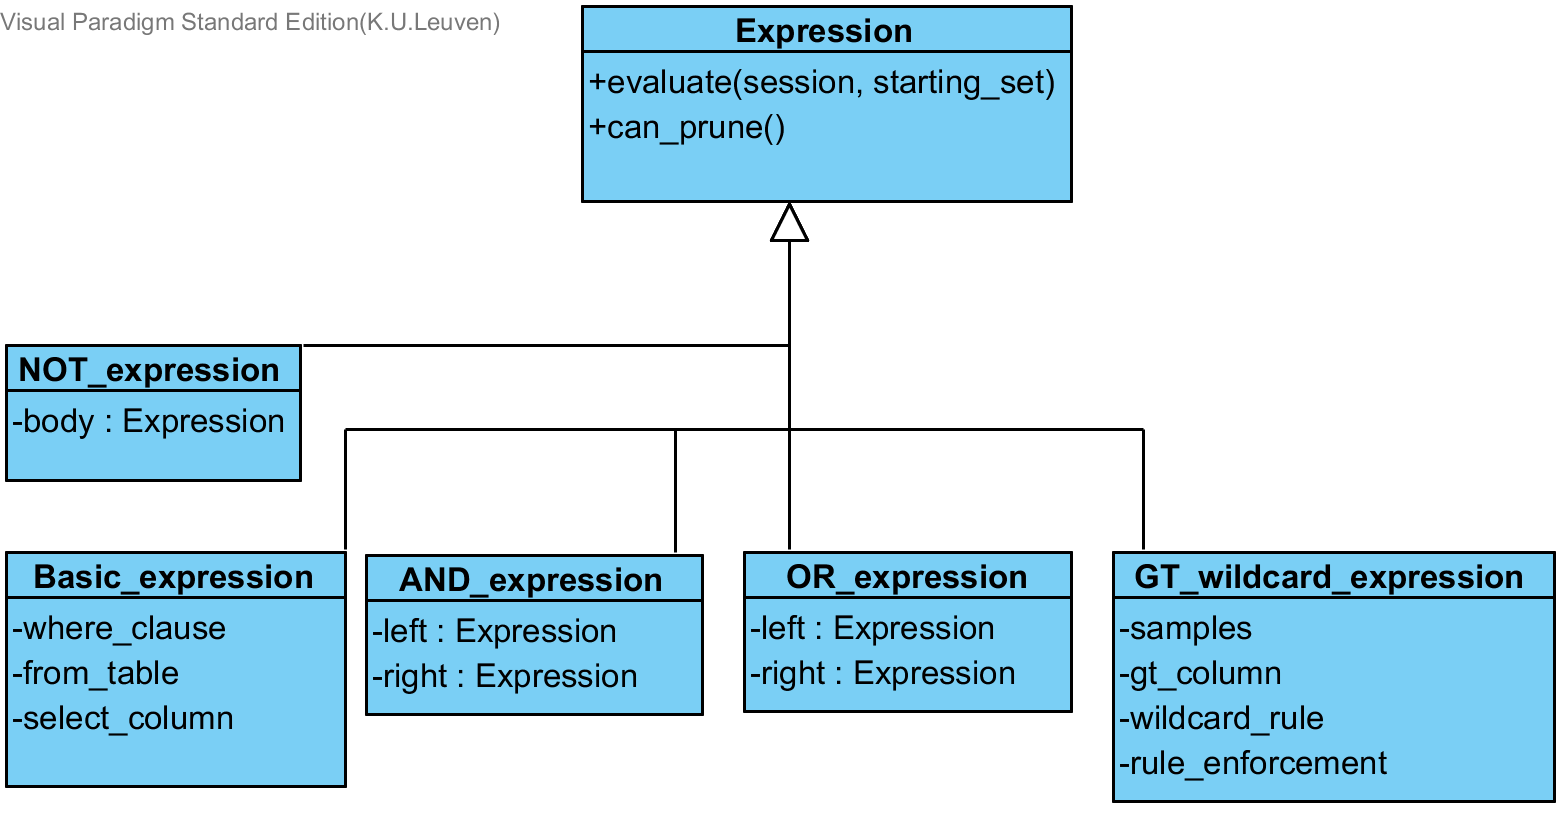
\includegraphics[width=\textwidth,height=\textheight,keepaspectratio]{query_exps}
\caption{De \texttt{query\_expressions} waarmee alle queries gemodelleerd worden. Het \texttt{session}-argument van de \texttt{evaluate}-functie is een actieve verbinding met het Cassandra-cluster.}
\label{query_exps_diagram}
\end{figure}

\subsection{Combineren subqueries}

Uit performantie-overwegingen is het een logische keuze de resultaten van subqueries op de hulptabellen te bewaren in een set datatype. Zo kunnen de benodigde set-operaties gebruik maken van de in Python ingebouwde set-operaties en zo veel effici\"enter verlopen dan wanneer de resultaten in bijvoorbeeld lists bewaard worden. Het enige nadeel van sets t.o.v. lists is dat de implementatie geen garanties biedt over in welke volgorde rijen in het eindresultaat zullen voorkomen. Dit weegt niet op tegen de tijdswinst, en bovendien biedt Cassandra zelf (in de algemeen aangeraden consistent hashing-partitionering) geen enkele garantie over in welke volgorde het rijen opslaat.\\\\
Bij het praktisch evalueren van \texttt{query\_expression}s komt uiteindelijk meer kijken dan enkel set-operaties. De belangrijkste reden hiervoor is dat, zoals in \ref{comb_subq_concept} reeds beschreven, om een negatie of \texttt{NOT\_expression} te kunnen evalueren, alle kandidaat-rijen gekend moet zijn, en dus meegegeven aan de \texttt{evaluate}-functie. Die extra informatie kan ook bij het evalueren van andere types van \texttt{query\_expression} goed van pas komen.
 
\begin{itemize}
\item Het evalueren van \texttt{Basic\_expression}s gebeurt niet zo rechtoe rechtaan als de naam doet vermoeden. De \texttt{evaluate}-functie bouwt een CQL-query op, op basis van een gegeven \texttt{WHERE}-clausule, de relevante tabel en de gevraagde kolom uit die tabel. Wanneer er een zinvolle verzameling kandidaatrijen (de \texttt{starting\_set} in onderstaand codefragment) meegegeven is, wordt die als \texttt{IN}-clausule aan de \texttt{WHERE}-clausule toegevoegd. Zo zoekt Cassandra enkel in rijen die effectief in aanmerking komen om aan de globale query te voldoen. Een voorwaarde om die optimalisatie te kunnen toepassen, is dat de \texttt{WHERE}-clausule geen ongelijkheidsbeperkingen mag bevatten (vandaar de \texttt{can\_prune}-functie).

\lstinputlisting[language=Python,firstline=31,lastline=48]{gemini_src/query_expressions.py}

\item Om een \texttt{AND\_expression} te evalueren is het strikt genomen nodig beide leden van de uitdrukking te evalueren en vervolgens de doorsnede te nemen van de resultaten. Als \'e\'en van de twee leden van de uitdrukking echter in staat is om dankzij een CQL \texttt{IN}-clausule enkel naar rijen te zoeken die effectief in aanmerking komen om aan de globale query te voldoen, is het mogelijk om die operatie aan Cassandra over te laten. Als het rechterlid kan \textit{prunen}, dan kan GEMINI de resultaatverzameling van het linkerlid als \texttt{starting\_set} meegeven bij de evaluatie van het rechterlid, en omgekeerd. Wanneer geen van beide kunnen \textit{prunen}, moet GEMINI uiteraard nog steeds zelf de doorsnede berekenen.

\lstinputlisting[language=Python,firstline=56,lastline=66]{gemini_src/query_expressions.py}

\item In het geval van een \texttt{OR\_expression} is er geen andere mogelijkheid dan eenvoudigweg het linker- en rechterlid te evalueren, beide met als \texttt{starting\_set} de \texttt{starting\_set} van de \texttt{OR\_expression} zelf, en vervolgens de unie van de resultaten te berekenen.

\item Ook in het geval van een \texttt{NOT\_expression} is er geen andere optie dan de \texttt{body}-uitdrukking te evalueren en vervolgens het complement van de \texttt{starting\_set} en het resultaat te bepalen. Als de gegeven \texttt{starting\_set} gelijk is aan \texttt{"*"}, d.w.z. alle rijen in de oorspronkelijke tabel, zit er ook niets anders op dan die nog eerst allemaal op te vragen.

\lstinputlisting[language=Python,firstline=101,lastline=110]{gemini_src/query_expressions.py}

\end{itemize}

Een optimalisatie die voor alle \texttt{query\_expressions} geldt is dat in het geval van een lege \texttt{starting\_set}, GEMINI de hele evaluatie kan overslaan. Dit bespaart een overtollige round-trip naar de Cassandra-databank. Voor alle soorten \texttt{query\_expressions} behalve de \texttt{Basic\_expression} geldt ook dat ze kunnen \textit{prunen}, ongeacht de aard van hun subqueries. In het geval dat hun subqueries een \texttt{Basic\_expression} bevatten die niet kan \textit{prunen}, zal de subquery in kwestie dit zelf afhandelen bij de evaluatie.

\subsection{Ophalen finaal resultaat}

Eens de primary keys van de rijen gekend zijn die voldoen aan de query, rest er enkel nog de gevraagde kolommen uit de hoofdtabel op te vragen uit de hoofdtabel. Voor deze laatste query op de hoofdtabel gebruikt onze implementatie de CQL \texttt{IN}-clausule om de primary keys te  specifi\"eren. Omdat een GEMINI-query al snel meerdere tienduizenden rijen oplevert, is het niet aangeraden die allemaal in \'e\'en gigantische \texttt{IN}-clausule op te vragen, om timeouts te vermijden. Het is dus zaak de verzameling primary keys in kleinere batches op te splitsen. Die batches kunnen dan ook over meerdere processoren verdeeld worden om zo een hogere leesthroughput te bereiken. Het enige nadeel van de parallellisatie is dat de verschillende processen niet meer effici\"ent naar eenzelfde output kunnen schrijven. Onze implementatie laat elke processor naar een apart bestand schrijven, die dan achteraf eventueel met elkaar geconcateneerd kunnen worden.

\subsection{Genotype-filter wildcards}
\label{gt_wildcards}

Gegeven het bovenstaande query-mechanisme is de meest voor de hand liggende manier om genotype-filter wildcards te implementeren, ze op te splitsen in subqueries voor elke sample die aan de voorwaarden in de \texttt{sample\_wildcard} voldoet, en die subqueries te combineren met een keten van geneste \texttt{query\_expression}s afhankelijk van de gegeven \texttt{rule\_enforcement}. Zo wordt een \texttt{all}-wildcard een keten van geneste \texttt{AND\_expression}s en een \texttt{any}-wildcard een keten van geneste \texttt{OR\_expression}s. \texttt{none}-wildcards vereisen eerst dat de subqueries in \texttt{NOT\_expression}d ingebed worden, die vervolgens allemaal in een keten van geneste \texttt{AND\_expression}s gecombineerd worden. Het is moeilijker \texttt{count}-wildcards tot dergelijke \texttt{expressions} om te vormen. Die vergen een aparte strategie, die later aan bod komt.\\
Deze aanpak is vergelijkbaar met wat er in de SQLite- en PostgresQL-versies van GEMINI gebeurt: in SQLite vormt GEMINI de wildcards om tot lange Python-expressions die uiteindelijk voor elke variant met de Python \texttt{eval()}-functie ge\"evalueerd worden. Dit uiteraard omdat de genotype-kolommen bestaan uit binary blobs die voor de SQLite-databank geen enkele betekenis hebben. De PostgreSQL-versie van GEMINI pakt het slimmer aan en vormt de wildcards om tot lange SQL \texttt{WHERE}-clausules en laat zo het evaluatiewerk over aan de databank, met de bemerking dat de PostgreSQL-versie \texttt{count}-wildcards vooralsnog niet ondersteunt omdat dit niet rechtstreeks in SQL vertaald kunnen worden.\\
In dit opzicht lijkt de Cassandra-implementatie op de SQLite-implementatie, gezien de client, niet de databank, het meeste werk verricht.\\

Zoals in de conceptuele uitleg van de oplossing aangehaald, kan de evaluatie van genotype-wildcards effici\"enter verlopen door de evaluatie van de subqueries in parallel uit te voeren op meerdere processoren. Dit hebben we ook daadwerkelijk ge\"implementeerd, door introductie van een nieuw type \texttt{query\_expression}, namelijk de \texttt{GT\_wildcard\_expression}.\\
Bij evaluatie zal die de namen van alle samples die aan de \texttt{sample\_wildcard} voldoen verdelen over het aantal processoren dat de gebruiker meegeeft, elke processor een tussenresultaat laten berekenen, de resultaten opvragen en samenvoegen m.b.v. de gekende setalgebra. Om het werk effici\"ent over verschillende processoren te verdelen en alle benodigde informatie te communiceren, maakt de implementatie gebruik van zogenaamde subprocesses, die elk hun eigen verbinding openen met het Cassandra-cluster, en interprocess-communicatiemechanismen uit de Python \texttt{multiprocessing}-API \cite{multiprocessing}.\\

\lstinputlisting[language=Python,firstline=173,lastline=197]{gemini_src/query_expressions.py}

\texttt{all-, any-} en \texttt{none-}wildcards vereisen voor het samenvoegen van de resultaten van de verschillende subprocesses geen grote aanpassingen aan de sequenti\"ele evaluatie-strategie van wildcards. Omdat die oplossingswijze er zich uitstekend toe leent af te wijken van het stramien van de geneste \texttt{query\_expressions} (immers, er is maar 1 \texttt{GT\_wildcard\_expression} voor alle samples), is het makkelijker de \texttt{count}-wildcards te implementeren: elk subprocess voert subqueries uit voor de samples waarvoor het verantwoordelijk is en telt voor elke variant hoe vaak hij in de resultaatverzamelingen van de subqueries voorkomt. Die informatie stuurt het subprocess terug naar zijn parent-process in een Python \textit{dictionary}, met een map van \texttt{variant\_id}s naar de telling.

\lstinputlisting[language=Python,firstline=315,lastline=341]{gemini_src/query_expressions.py}

Het parent-process kan vervolgens de telling voor alle variants van alle subprocesses bij elkaar optellen, en met gebruik van de Python \texttt{eval}-functie alle variants die aan de \texttt{count}-filter voldoen, bepalen. Let wel, bij het opstellen van de uiteindelijke \textit{dictionary} met de tellingen voor de varianten, moet het parent-process voor alle varianten in de \texttt{starting\_set}, een entry voorzien, met defaultwaarde 0. Zoniet zullen varianten waarvoor geen enkele sample aan de \texttt{gt\_wildcard\_rule} voldoet, niet in het resultaat voorkomen, en \texttt{count}-filters als \texttt{(count < x), (count <= x)} (voor arbitraire, positieve \texttt{x}) of \texttt{(count == 0)}  die varianten onterecht niet in hun resultaat weergeven.

\lstinputlisting[language=Python,firstline=212,lastline=222]{gemini_src/query_expressions.py}

\noindent De \texttt{correct\_starting\_set} in bovenstaande code is de traditionele \texttt{starting\_set}, maar ge\"evalueerd in het geval dit de volledige verzameling varianten (dus de wildcard \texttt{"*"}) is, en gegoten in een datatype geschikt voor shared-memory access.\\
De \texttt{invert\_count}-flag geeft aan of de \texttt{gt\_wildcard\_rule} een negatie is. Gezien Cassandra geen \texttt{!=}-clausules ondersteunt, moet GEMINI in dit geval het complement van de \texttt{gt\_wildcard\_rule} in kwestie bepalen en vervolgens de resulterende telling aftrekken van het totaal aantal samples. \\ Een eenvoudig voorbeeld: bij het evalueren van volgende wildcard \\\\ 
\texttt{(gt\_type).(*).(!=HET).(count > 100)}\\\\
zal GEMINI eerst voor elke variant bepalen hoeveel samples w\'el heterozygoot zijn, alvorens dit getal af te trekken van het totaal aantal samples en op dit resultaat de \texttt{(count > 100)}-filter toe te passen.

\section{Implementatie: conclusies}

De implementatie van het ontwerp beschreven in hoofdstuk \ref{concept} vergt vooral ingrijpende wijzigingen aan het queryingmechanisme van GEMINI: ons ontwerp analyseert queries at runtime, splitst \texttt{WHERE}-clausules en genotype-filters en -wildcards op in meerdere subqueries tegen de Cassandra databank en combineert de resultaten van die subqueries tot een coherent resultaat met behulp van set-arithmetiek. De evaluatie van de subqueries kan in parallel gebeuren op meerdere processoren om het gehele proces sneller te laten verlopen.\\
Aan het mechanisme om genoominformatie in te laden in GEMINI verandert er minder. Ook die taak kan dankzij Cassandra eenvoudig geparalleliseerd worden, door meerdere processoren los van elkaar een disjunct deel van de data in te laten laden, rechtstreeks in dezelfde Cassandra databank.
